%!TEX root = ../report.tex

% 
% Architecture
% 

\section{Solution's Architecture Proposal}

Considering this project's problem and the objectives presented in problem contextualization section, we want to develop a process architecture for project and maintenance management to be applied to an Information Systems administration, supported by a logical application architecture.\par
As long as this project is aligned with a real-case scenario for an organization, we will take the main design decisions considering the stakeholders' needs and concerns for this project, namely the processes to consider for the architecture development and the solutions chosen for integrating the logical application architecture. It will also provide a demonstration scenario for our solution, allowing us to achieve the demonstration and evaluation steps of the DSRM process.\par 



\subsection{Real-case Scenario}

The real-case organization scenario will provide constraints and assumptions for this project, made available by the organization's stakeholders. Being so, some design decisions were made considering specific requirements from this scenario.\par
We are dealing with an organization from the utilities sector of Business (Energy), composed by a unique administration for Applications (software) area. This administration will receive two types of requests: project execution and evolving maintenance requests.\par
Considering the stakeholders for this project, we have two types: Internal and External. Considering internal stakeholders, we have the Business area, composed by the organization administration (Sponsor of this project), the financial and logistic departments, and the Technology area, composed by the Information Systems department (Project execution and Maintenance departments). Considering the external stakeholders, we have the third-parties responsible for project implementation, suppliers, consumers and regulatory entities.\par
Project Execution department will outsource project implementation to a third-party but internally will maintain processes for project management, independent from the third-party. Evolving maintenance requests are filtered by a Help-Desk service, Wherefore only the major changes requests arrive to the evolving maintenance department.\par
A project only enters in production phase after approval from the maintenance department. When in production phase, project belongs to the maintenance department. It can, accordingly with a strategical plan previously defined, outsource the maintenance's implementation, being only responsible for its management.\par
This real-case scenario will allow us to extract some requirements and also take design decisions accordingly to organization's stakeholders' needs and concerns, deciding which processes must be included in the processes architecture and the ones we should not focus, to reduce unnecessary complexity.\par


\subsection{Process Architecture}

Taking as reference ISO/IEC 12207, detailed in section 5.1, that standardizes the processes for the whole life cycle of software, we will present the areas we will address in our processes architecture and the reasons for not considering others.\par
The two main processes areas we can address are governance and management processes. Considering the extensibility of both, we could not focus on the two, giving the time-frame available. Being so, we decided, accordingly with the stakeholders, to not detail governance processes. This type of processes need maturation and organization's insight, being too much complex in the scope of this project. Areas as organization strategy or project portfolio will not be addressed.\par 
Despite this, there are governance processes that will have direct influence on the subjects covered by this project, namely risk, budget and quality management. These subjects will be addressed considering a more operational approach, assuming that organization's strategy for this areas is already defined, being our mission design processes that implement it in practice.\par
We are considering the use of BPMN 2.0 (Business Process Model and Notation) for processes modeling. It provides a graphical representation for specifying business processes, being the standard for business processes modeling. Due to its large adoption by organizations for business processes' specification, it is the best option for designing a processes architecture. \par


\subsubsection{Processes definition}

Using an interview approach with the organization's stakeholders for a more deeper analysis on the problem scope, we defined the areas of interest we need to cover. This areas can change during project execution phases, since requirements are volatile and can be changed. Also, more areas can be covered in the future, if we consider it brings an added value for this architecture.\par
In Figure 18 we can observe the processes of interest for this project highlighted from the ISO/IEC 12207 international standard. As explained before, processes directly related to governance areas are not considered for this project due to its increased complexity. As consequence, Agreement processes and Organizational Project-Enabling processes are outside the scope for this project.\par
Technical Processes and Software Implementation processes are also not considered in the scope, based on the requirements presented by the stakeholders and the organization scenario provided. As stated in section 7.1, we will assume these processes will be either outsourced, or managed by the organization according to already defined processes for that purpose.\par
Software Reuse Processes are also outside the scope of this project. It is a shared opinion of stakeholders that this processes are not related to this project's problem and would only increase its complexity without adding any value.\par
The processes we will address in detail are the Project processes and the Software Support processes, directly related to project and maintenance management. It constitutes the core of this project and is fundamental for establishing the proposed processes architecture.\par
Regarding Project processes, and accordingly to the concerns extracted from the stakeholders' interview, we will consider all processes with exception of configuration management process and measurement process, that are not in the scope of interest for this particular project. Considering Software Support Processes, we will only address the Software Configuration Management process and the Software Validation process.\par


\begin{figure}[h!]
\centering
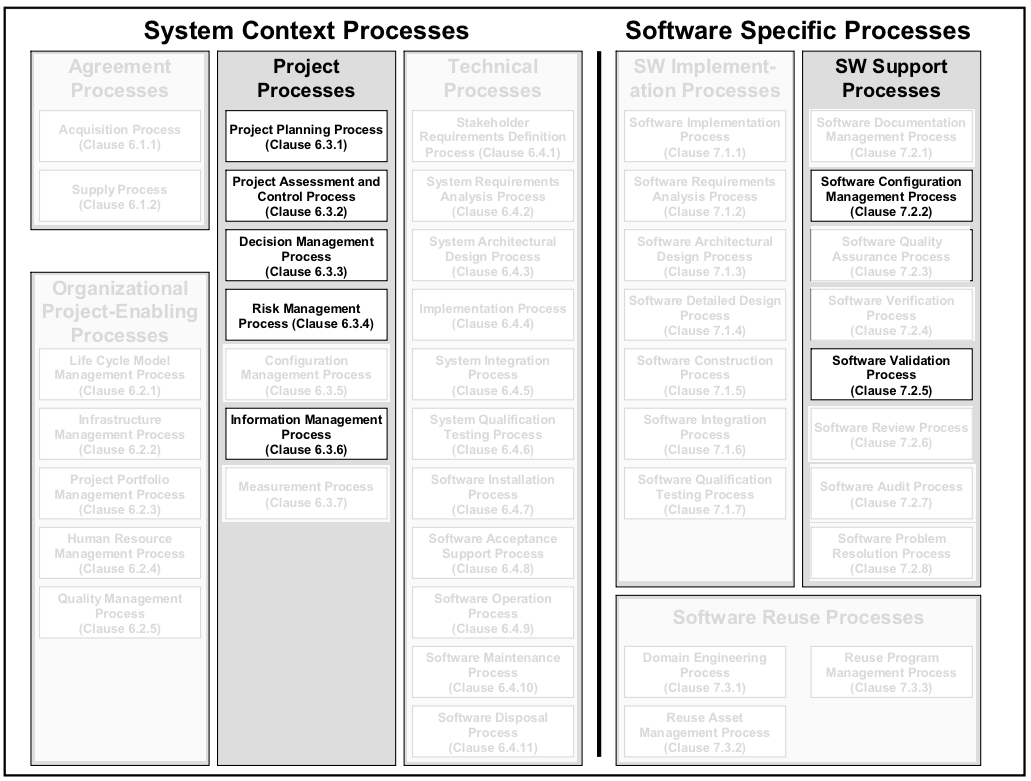
\includegraphics[width=0.8\textwidth]{img/ISO12207ProcessesImplemented.png}
\caption{Processes areas considered for this project. Adapted from \cite{ISO12207}.}
\end{figure}

Apart from processes presented by ISO/IEC 12207, the stakeholders presented specific concerns regarding processes on Capacity Management, Issues Management, Financial Management and Document Management. They need to be taking in account on this project's scope considering stakeholders' needs.\par
Capacity Management, as stated in \cite{itilSD}, ``ensure that cost-justifiable IT capacity in all areas of IT always exists and is matched to the current and future agreed needs of the business, in a timely manner.''. Deals with performance achievement and capacity availability, considering resources and services itself. It tries to balance costs against resources needed and supply against demand.\par
The main areas are Business Capacity Management (requirements for service and IT infrastructure), Service Capacity Management (performance and capacity management of IT services operation) and Component Capacity Management (performance, capacity and utilization management of individual IT technology components).\par
Issues Management is the process of identifying and resolving issues, as staff, suppliers, technical or material problems. Many times confused with risks, they can arise from project processes with no warning or no expectation at all. Most organizations find difficult to manage issues from an effectively manner and many times it a process that is not implemented across the complete organization, making more difficult its resolution.\par
Financial Management, as stated in \cite{itilSS}, ``provides the business and IT with the quantification, in financial terms, of the value of IT Services, the value of the assets underlying the provisioning of those services, and the qualification of operational forecasting''. Core areas for IT Financial Management are Budgeting (Expenditures planning and controlling), IT accounting (Cost analysis on IT services providing) and Charging (Costs assignment to IT services provided). Financial Management is a complex area and we need a more deeper analysis on its importance for our architecture, in order to remove unnecessary complexity.\par
Documentation Management corresponds to an area that deals with all documentation concerns on an organization, from technical to project management documentation. This area groups processes for plan, production, tracking and communication of documents produced by the organization in project and maintenance contexts. This processes are also related to the supporting artifacts we want to develop.\par
In Table 2 we present the processes we will consider for this project and a description of some activities each process implements.

\begin{table}[h!]
\centering
\resizebox{0.9\textwidth}{!}{%
\begin{tabular}{|c|l|}
\hline
\textbf{Processes} & \multicolumn{1}{c|}{\textbf{Description}} \\ \hline
\textbf{Project Planning} & \begin{tabular}[c]{@{}l@{}}Scope and goals definition;\\ Requirements establishment;\\ Activities and deliverables identification;\\ Schedule definition;\\ Resources identification;\\ Responsibilities assignment;\\ Quality, Risk and Cost Analysis;\end{tabular} \\ \hline
\textbf{Project Assessment and Control} & \begin{tabular}[c]{@{}l@{}}Project monitoring;\\ Project control;\\ Project assessment;\end{tabular} \\ \hline
\textbf{Decision Management} & \begin{tabular}[c]{@{}l@{}}Decision Planning;\\ Decision analysis;\\ Decision tracking;\end{tabular} \\ \hline
\textbf{Risk Management} & \begin{tabular}[c]{@{}l@{}}Risk Management planning;\\ Risk Profile Management;\\ Risk Analysis;\\ Risk Treatment;\\ Risk Monitoring;\\ Risk Management process evaluation;\end{tabular} \\ \hline
\textbf{Capacity Management} & \begin{tabular}[c]{@{}l@{}}Capacity Plan definition;\\ Performance Monitoring;\\ Performance Analysis;\\ Performance tuning;\end{tabular} \\ \hline
\textbf{Issues Management} & \begin{tabular}[c]{@{}l@{}}Issue Identification;\\ Issue Prioritization;\\ Issue Resolution;\\ Issue Communication;\end{tabular} \\ \hline
\textbf{Financial Management} & \begin{tabular}[c]{@{}l@{}}Budgeting definition;\\ IT Accounting planning;\\ Charging planning;\\ Financial control;\\ Financial communication;\end{tabular} \\ \hline
\textbf{Documentation Management} & \begin{tabular}[c]{@{}l@{}}Documentation definition;\\ Documentation production;\\ Documentation validation;\\ Documentation communication;\\ Documentation tracking;\end{tabular} \\ \hline
\textbf{Software Configuration Management} & \begin{tabular}[c]{@{}l@{}}Software configuration management plan developing;\\ Configuration Identification;\\ Configuration Control;\\ Configuration Status Accounting;\\ Configuration Evaluation;\end{tabular} \\ \hline
\textbf{Software Validation} & \begin{tabular}[c]{@{}l@{}}Validation plan definition;\\ Test requirements, test cases and test specifications preparation;\\ Tests Execution;\\ Software validation against the requirements execution;\end{tabular} \\ \hline
\end{tabular}
}
\vspace{2mm}
\caption{Processes areas and main activities.}
\label{my-label}
\end{table}



\subsubsection{Processes Mapping to frameworks}

In this section we will present how each one of the processes in the scope for this project is addressed and mapped into the frameworks and standards presented in section 4 and 5. This will provide us an initial guidance on how we should approach the problem, analyzing what objectives are already covered by the frameworks and which ones need more original work.\par
Our objective is to use only the important knowledge from sections 4 and 5 for this project, reducing the complexity of implementing a complete framework for the organization. In Table 3 we present the mapping between each processes group in the scope for this project with the framework or standard that covers some aspects for it:\par

\begin{table}[h!]
\centering
\resizebox{\textwidth}{!}{%
\begin{tabular}{|l|c|c|c|c|c|c|c|c|c|c|c|c|c|}
\hline
\multicolumn{1}{|c|}{} & \multicolumn{4}{c|}{\textbf{COBIT 5 Domains}} & \multicolumn{5}{c|}{\textbf{ITIL V3 Volumes}} &  &  &  &  \\ \cline{2-10}
\multicolumn{1}{|c|}{\multirow{-2}{*}{\textbf{Processes}}} & \textbf{APO} & \textbf{BAI} & \textbf{DSS} & \textbf{MEA} & \textbf{SS} & \textbf{SD} & \textbf{SO} & \textbf{ST} & \textbf{CSI} & \multirow{-2}{*}{\textbf{PMBOK}} & \multirow{-2}{*}{\textbf{\begin{tabular}[c]{@{}c@{}}ISO/IEC\\ 20000\end{tabular}}} & \multirow{-2}{*}{\textbf{\begin{tabular}[c]{@{}c@{}}ISO/IEC \\ 27000\end{tabular}}} & \multirow{-2}{*}{\textbf{\begin{tabular}[c]{@{}c@{}}ISO\\ 31000\end{tabular}}} \\ \hline
\textbf{Project Planning} & \cellcolor[HTML]{5A9D58}\checkmark & \cellcolor[HTML]{5A9D58}\checkmark &  &  &  &  &  &  &  & \cellcolor[HTML]{FD6864}\checkmark & \cellcolor[HTML]{329A9D}\checkmark &  &  \\ \hline
\textbf{Project Assessment and Control} & \cellcolor[HTML]{5A9D58}{\color[HTML]{000000} \checkmark} & \cellcolor[HTML]{5A9D58}{\color[HTML]{000000} \checkmark} & \cellcolor[HTML]{5A9D58}{\color[HTML]{000000} \checkmark} & \cellcolor[HTML]{5A9D58}{\color[HTML]{000000} \checkmark} &  &  &  &  &  & \cellcolor[HTML]{FD6864}\checkmark & \cellcolor[HTML]{329A9D}\checkmark &  &  \\ \hline
\textbf{Decision Management} & \cellcolor[HTML]{5A9D58}{\color[HTML]{000000} \checkmark} & \cellcolor[HTML]{5A9D58}{\color[HTML]{000000} \checkmark} & \cellcolor[HTML]{5A9D58}{\color[HTML]{000000} \checkmark} & \cellcolor[HTML]{5A9D58}{\color[HTML]{000000} \checkmark} & \cellcolor[HTML]{FFCC67}\checkmark &  &  &  &  & \cellcolor[HTML]{FD6864}\checkmark & \cellcolor[HTML]{329A9D}\checkmark &  &  \\ \hline
\textbf{Risk Management} & \cellcolor[HTML]{5A9D58}\checkmark &  &  &  &  & \cellcolor[HTML]{FFCC67}\checkmark &  &  &  & \cellcolor[HTML]{FD6864}\checkmark &  & \cellcolor[HTML]{329A9D}\checkmark & \cellcolor[HTML]{329A9D}\checkmark \\ \hline
\textbf{Capacity Management} & \cellcolor[HTML]{5A9D58}\checkmark & \cellcolor[HTML]{5A9D58}\checkmark &  &  &  & \cellcolor[HTML]{FFCC67}\checkmark &  &  &  &  &  &  &  \\ \hline
\textbf{Issues Management} &  &  & \cellcolor[HTML]{5A9D58}\checkmark &  &  &  & \cellcolor[HTML]{FFCC67}\checkmark &  &  &  &  &  &  \\ \hline
\textbf{Financial Management} & \cellcolor[HTML]{5A9D58}\checkmark &  &  &  & \cellcolor[HTML]{FFCC67}\checkmark &  &  &  &  &  &  &  &  \\ \hline
\textbf{Documentation Management} & \cellcolor[HTML]{5A9D58}\checkmark & \cellcolor[HTML]{5A9D58}\checkmark &  &  &  &  &  &  &  & \cellcolor[HTML]{FD6864}\checkmark &  & \cellcolor[HTML]{329A9D}\checkmark &  \\ \hline
\textbf{Software Configuration Management} &  & \cellcolor[HTML]{5A9D58}\checkmark &  &  &  &  &  & \cellcolor[HTML]{FFCC67}\checkmark &  &  &  &  &  \\ \hline
\textbf{Software Validation} & \cellcolor[HTML]{5A9D58}\checkmark &  &  &  &  &  &  & \cellcolor[HTML]{FFCC67}\checkmark &  & \cellcolor[HTML]{FD6864}\checkmark &  &  &  \\ \hline
\end{tabular}
}
\vspace{2mm}
\caption{Processes Mapping to frameworks and standards.}
\label{my-label}
\end{table}


\subsubsection{Processes Supporting artifacts}

Considering the processes architecture we want to develop, we need some artifacts to support this processes, namely communication and decisions artifacts that will allow us to support the activities' inputs and outputs. For this, we will identify all artifacts needed, clearly defining its purpose, content and participants.\par
This artifacts will be defined during the designing of the process architecture. The frameworks and standards previously presented define some of them, being our work to address new artifacts that are not already covered and adapt others to better suit to our objectives.\par

\subsubsection{Responsibility Structure}

The developed architecture needs to have an inherent responsibility structure, defining the processes' participants accounted for decisions and activities. This structure is particularly important when considering we are dealing with a real-case organization, having an organizational structure already defined and for which our processes should be applied.\par
For designing this responsibility structure we will consider the work already done in responsibility assignment for the frameworks and standards previously presented. Despite that, we need also to have some original work on this area, considering we are not implementing directly any of those frameworks. This work will be accomplished during the processes' design and taking in account the common responsibility structures on IT organizations.\par 

\subsection{Logical Application Architecture}

A proposal for a logical application architecture is one of the objectives of this project, being important to support the processes architecture. To achieve this, we evaluated a set of PPM and ITSM solutions available in the market with the objective of achieving a proposal of applications that can be a part of this architecture.\par
We will only consider proprietary solutions, due to explicit requirements from the organization's stakeholders. This was a precondition that we did not take in account in the state of the art on section 6 but that in this phase will restrict our PPM and ITSM solutions' proposal.\par 
For evaluation purposes, we used Gartner and Forrester research, presented in section 6, that allow us to independently evaluate how these tools stand a position in the PPM and ITSM Market and also what are the solutions more complete in terms of features and capabilities.\par
In this section we will present the solutions we consider the best for our objectives, being part of a proposal for the project's stakeholders. After deciding what solution we will consider for this project, we need to design a logical application architecture, describing how processes are supported and integrated.\par

\subsubsection{PPM Tools}

For PPM solutions, that we evaluate in section 6.2, we used the Gartner Magic Quadrant and the Forrester Wave methodologies for evaluation.\par
In Magic Quadrant results, that performs an evaluation of the PPM solutions' providers adequacy to the market, we will just consider the leaders quadrant, composed by Planview, Compuware, CA, HP, Oracle and Microsoft. Planview and CA are the suppliers with the best results but are closely followed by the rest. A deeper analysis on strengths and cautions presented by Gartner for each one of this solutions is presented in \cite{magicQuadrantPPM}.\par
For the Forrester Wave results, that evaluates providers by criteria and respective weightings, we will consider the two models explained in section 6.2.2, the above-the-line and below-the-line. For the first one, the leaders quadrant is composed by Planview, CA Technologies, HP and Daptiv. All presents good results but is CA Technologies who is the most complete provider, in terms of current offering, strategy and market presence. Other providers present better results in some of this criteria but are substantially worse in others. For the below-the-line evaluation, we have CA Technologies and Planview very close to each other and HP with an excellent result in strategy criteria. Microsoft, Rally and Daptiv are also part of the leaders, but with results slightly worse.\par
In Table 3 we can observe the PPM Tools Evaluation results. In green we have the solutions we consider the best for this project taking in account the evaluation results. We also present the alternatives in orange. CA Technologies with CA Clarity PPM, Planview with Planview Enterprise and HP with HP PPM Center are the solutions we will purpose for the PPM Tool to consider for this project.


\begin{table}[h!]
\centering
\resizebox{\textwidth}{!}{%
\begin{tabular}{|c|c|l|c|c|l|}
\hline
 & \multicolumn{2}{c|}{} & \multicolumn{3}{c|}{\textbf{Forrester Wave}} \\ \cline{4-6} 
\multirow{-2}{*}{\textbf{Solutions Providers}} & \multicolumn{2}{c|}{\multirow{-2}{*}{\textbf{\begin{tabular}[c]{@{}c@{}}Gartner Magic\\ Quadrant\end{tabular}}}} & \multicolumn{1}{l|}{\textbf{Above-The-Line}} & \multicolumn{2}{l|}{\textbf{Below-The-Line}} \\ \hline
\rowcolor[HTML]{5A9D58} 
\textbf{CA Technologies} & \multicolumn{2}{c|}{\cellcolor[HTML]{5A9D58}Leader} & Leader & \multicolumn{2}{c|}{\cellcolor[HTML]{5A9D58}Leader} \\ \hline
\rowcolor[HTML]{5A9D58} 
\textbf{Planview} & \multicolumn{2}{c|}{\cellcolor[HTML]{5A9D58}Leader} & Leader & \multicolumn{2}{c|}{\cellcolor[HTML]{5A9D58}Leader} \\ \hline
\rowcolor[HTML]{5A9D58} 
\textbf{HP} & \multicolumn{2}{c|}{\cellcolor[HTML]{5A9D58}Leader} & Leader & \multicolumn{2}{c|}{\cellcolor[HTML]{5A9D58}Leader} \\ \hline
\rowcolor[HTML]{FFCB2F} 
\textbf{Microsoft} & \multicolumn{2}{c|}{\cellcolor[HTML]{FFCB2F}Leader} & Strong Performer & \multicolumn{2}{c|}{\cellcolor[HTML]{FFCB2F}Leader} \\ \hline
\textbf{Oracle} & \multicolumn{2}{c|}{Leader} & - & \multicolumn{2}{c|}{-} \\ \hline
\textbf{Compuware} & \multicolumn{2}{c|}{Leader} & - & \multicolumn{2}{c|}{-} \\ \hline
\textbf{Rally} & \multicolumn{2}{c|}{-} & Strong Performer & \multicolumn{2}{c|}{Leader} \\ \hline
\textbf{Daptiv} & \multicolumn{2}{c|}{-} & Leader & \multicolumn{2}{c|}{Leader} \\ \hline
\end{tabular}
}
\vspace{2mm}
\caption{PPM Tools evaluation results.}
\label{my-label}
\end{table}

\vspace{10mm}

\subsubsection{ITSM Tools}

For ITSM solutions, that we evaluated in section 6.3, we used the Magic Quadrant , the Critical Capabilities and the Forrester Wave methodologies for evaluation.\par
In Magic Quadrant results we will just consider the leaders and challengers quadrants, composed by ServiceNow and BMC Software for the leaders and Cherwell and CA Technologies for challengers. ServiceNow is the best provider in terms of ability to execute with some advantage to concurrency but really close of BMC Software in terms of completeness of vision. Cherwell Software and CA Technologies present a considering lower result for completeness of vision considering the leaders quadrant. A deeper analysis on strengths and cautions presented by Gartner for each one of this solutions is presented in \cite{magicQuadrantITSM}.\par
In Critical Capabilities results, we will only consider the High-Maturity, Digital Workplace and Total ITSM Use Cases, the ones that are more adequate to our objectives and to the organization's scenario. We will also only consider the solutions provided by the suppliers in the leaders and challengers quadrants presented by Gartner. In all the use cases considered, BMC Remedy ITSM Suite and ServiceNow IT Service Automation suite have the higher scores, being followed by some distance by CA Service Management and Cherwell Software Service Management.\par
For the Forrester Wave results, we have Cherwell Software and Service Now as the leaders, very close to each other and with a very good result in terms of market presence. BMC Software and CA Technologies are considered Strong Performers, but at some distance of the other two. Forrester establishes big differences between the two leaders providers and the two strong contenders in terms of the three criteria considered.\par
In Table 4 we can observe the ITSM Tools Evaluation results. In green we have the solution we consider the best for this project taking in account the evaluation results. ServiceNow with ServiceNow IT Service Automation is the solution we will purpose for the ITSM Tool to consider for this project. We also present other alternatives in orange. It should be taken special attention to CA Technologies tool as alternative solution if we consider the CA Technologies PPM tool due to easier integration between the PPM and ITSM tools.\par


\begin{table}[h!]
\centering
\resizebox{\textwidth}{!}{%
\begin{tabular}{|c|c|c|c|c|c|}
\hline
 &  & \multicolumn{3}{c|}{\textbf{Gartner Critical Capabilities}} &  \\ \cline{3-5}
\multirow{-2}{*}{\textbf{\begin{tabular}[c]{@{}c@{}}Solutions\\ Providers\end{tabular}}} & \multirow{-2}{*}{\textbf{\begin{tabular}[c]{@{}c@{}}Gartner\\ Magic \\ Quadrant\end{tabular}}} & \textbf{\begin{tabular}[c]{@{}c@{}}High\\ Maturity\\ UC\end{tabular}} & \textbf{\begin{tabular}[c]{@{}c@{}}Digital \\ Workplace \\ UC\end{tabular}} & \textbf{\begin{tabular}[c]{@{}c@{}}Total\\  ITSM\\ Use Case\end{tabular}} & \multirow{-2}{*}{\textbf{\begin{tabular}[c]{@{}c@{}}Forrester \\ Wave\end{tabular}}} \\ \hline
\rowcolor[HTML]{5A9D58} 
\textbf{ServiceNow} & Leaders & 3,68 & 3,49 & 3,56 & Leader \\ \hline
\rowcolor[HTML]{FFCC67} 
\textbf{Cherwell Software} & Challengers & 3,15 & 3,12 & 3,22 & Leader \\ \hline
\rowcolor[HTML]{FFCC67} 
\textbf{BMC Software} & Leaders & 3,74 & 3,49 & 3,52 & Strong Performers \\ \hline
\rowcolor[HTML]{FFCC67} 
\textbf{CA Technologies} & Challengers & 3,39 & 3,31 & 3,22 & Strong Performers \\ \hline
\end{tabular}
}
\vspace{2mm}
\caption{ITSM Tools evaluation results.}
\label{my-label}
\end{table}

